%----------------------------------------------------------------------
%                        PROJECT DEFINITION
%----------------------------------------------------------------------
\renewcommand{\projnr}{B1}
\renewcommand{\projtitleshort}{Charge transfer}
\renewcommand{\projauth}{Blum, Wurm}
%
\setcounter{section}{0}
\noindent{\normalfont\sffamily\Large\bfseries Project \projnr: \projtitleshort}
%
\section{Full title:}
\hspace{1\baselineskip}\\
\centerline{\large ``Charge transfer in dust-agglomerate
collisions}\\
\centerline{\large and the efficiency of electrostatic secondary agglomeration''}
%
\section{General information}\mbox{}
\subsection{Principle investigators:}
\hspace{-\baselineskip}\\\noindent
%
{\bfseries\itshape Blum}, J\"urgen, Prof.~Dr.\\
C3, tenure\\
Date-of-birth: 05. April 1962, Nationality: German\\
DFG Code number of latest application: Bl 298-6/2\\
Institut f\"ur Geophysik und extraterrestrische Physik\\
Mendelssohnstr.~3\\
38106 Braunschweig\\
Tel: 0531 391 5217\\
Fax: 0531 391 8126\\
Email: j.blum@tu-bs.de\\
Private address: Wendenring 14, 38114 Braunschweig, Tel: 0531 1216432\\
%
\vspace{1em}\\\noindent
{\bfseries\itshape Wurm}, Gerhard, Dr.\\
Leader Emmy Noether research group, non-tenure\\
Date-of-birth: 05. April 1967, Nationality: German\\
DFG Code number of latest application: WU 321/2-4\\
Institut f\"ur Planetologie\\
Wilhelm-Klemm-Str.~10\\
48149 M\"unster\\
Tel: 0251 8339052\\
Fax: 0251 8336301\\
E-mail: gwurm@uni-muenster.de\\
Private address: Kesslerweg 50d, 48155 M\"unster, Tel: 0251
6279418\\

\subsection{Co-investigators within this Forschergruppe:}
\begin{coilist}
\item W.~Kley (TAT/CPT, Univ. T\"ubingen)
\item U.~Motschmann (ITP, TU Braunschweig)
\item C.P.~Dullemond (MPIA Heidelberg)
\item H.~Klahr (MPIA Heidelberg)
\end{coilist}


\section{Summary (Zusammenfassung)}
\subsubsection{Summary:}
A possible explanation for a rapid formation of macroscopic bodies
in protoplanetary disks in spite of low sticking probabilities is
based upon the charge separation in non-sticking collisions. Such
a charge separation was observed in laboratory collisions between
microscopic dust particles and macroscopic solid targets. A
succession of non-sticking collisions can lead to the build-up of
surface charges and, thus, of strong electric fields on the larger
bodies from which emerging, previously non-sticking dust particles
are not able to escape. The proposed project aims at the
experimental test of this concept and the modelling of the
charge-induced growth of protoplanetary bodies. In addition to
that, chondrule-formation theories based on nebular lightning will
be tested.

\subsubsection{Zusammenfassung:}
Eine m\"ogliche Erkl\"arung f\"ur die schnelle Bildung
makroskopisch gro{\ss}er K\"orper in protoplanetaren Scheiben
trotz niedriger Haftwahrscheinlichkeiten basiert auf dem Effekt
der Ladungstrennung in nicht-haftenden Kollisionen. Eine solche
Ladungstrennung wurde bei Sto{\ss}versuchen zwischen mikroskopisch
kleinen Staubpartikeln und makroskopischen Fest\-k\"or\-pern
beobachtet. Eine Abfolge nicht-haftender St\"o{\ss}e kann zur
Ausbildung starker Oberfl\"a\-chen\-auf\-ladung und damit auch
starker elektrische Felder f\"uhren, die abprallende Staubpartikel
am Entweichen hindern. Das vorgeschlagene Projekt zielt darauf ab,
dieses Konzept experimentell zu \"uberpr\"ufen und das
ladungsinduzierte Wachstum protoplanetarer K\"orper zu
modellieren. Zus\"atzlich sollen Theorien zur Chondrenbildung, die
auf Blitzentladungen im protopla\-ne\-taren Nebel basieren,
getestet werden.

\section{State of the art (Stand der Forschung)}
The formation of planetesimals is still an open question. This is
in part due to the fact that the outcome of dust-dust collisions
has not been properly mapped. However, as compared to a decade
ago, we now have a much better view of the formation of
centimeter- to decimeter-sized protoplanetary bodies. This stage
was outlined by Weidenschilling \& Cuzzi (1993) for the
terrestrial-planet region and by Weidenschilling (1997) for the
outer regions of the solar nebula. The initially
(sub-)micrometer-sized dust (or ice) particles collide due to
Brownian motion and drift motions with respect to the nebular gas.
When the collision velocities are very low, i.e.\ for the initial
growth stage, each collision results in the immediate sticking of
the two colliding objects. Such hit-and-stick collisions lead to
the formation of fractal dust agglomerates with rather narrow size
distributions. As the surface-to-mass ratio of fractal dust
agglomerates does not change considerably with increasing
aggregate mass, the collision velocities (which are caused by
friction effects with the gas and are, thus, dependent on the
surface-to-mass ratio) remain basically constant. However, each
collision between a pair of fractal dust aggregates results in the
contact between two (sub-)micrometer-sized dust grains (one dust
grain from each aggregate) so that the increasing impact energy
(due to the growing dust-aggregate masses) leads to a rolling,
sliding, or breaking of the initiated grain-grain contact (Dominik
\& Tielens 1997). Ultimately, this leads to the compaction of the
dust aggregates and to the formation of non-fractal (but still
very porous) dusty bodies. When this happens, the non-fractal
aggregates start to drift much faster due to their decreased
surface-to-mass ratio so that they preferentially collide with
smaller or fractal dust aggregates. Finally, when the dust
aggregates grow beyond a certain size, their mean collision
velocities are so large that impacts no longer result in mass
gain. This stage is reached for centimeter- to decimeter-sized
bodies at 1 AU distance from the young sun.
\par
The subsequent growth stages of protoplanetary bodies are rather
speculative. We will briefly outline some of the current ideas on
planetesimal formation. (1) Wurm et al.\ (2001) showed that
collision-generated fragments can be aerodynamically trapped by
the larger body due to a systematic relative velocity between dust
and gas. Although this effect is restricted to bodies that are
smaller than the mean free path of the gas molecules (Sekiya \&
Takeda 2003, Wurm et al.\ 2004) showed that some of the fragments
can still be captured by larger bodies if they have a
non-vanishing gas permeability. (2) An alternative scenario, which
is the basis of the here-proposed project was outlined by Blum
(2004). Earlier laboratory experiments (see next section) showed
that impacts between dust particles and macroscopic solid bodies
lead to a systematic charge separation, even if the two colliding
bodies consist of identical materials (Poppe et al.~2000b; Poppe
\& Schr\"apler 2005). The number of separated elementary charges
increases roughly proportional to the impact energy so that exactly those
collisions that do not result in immediate sticking cause a strong
systematic charging. If the impact-charging process is more effective than
any discharging in the nebular gas, the larger bodies will accumulate
surface charges which lead to the formation of strong electric
fields\footnote{Charge separation on a macroscopic scale can lead to
electrical discharges in the nebula gas (Whipple \cit{1966}; Morfill et
al.~1993; Gibbard et al.~1997), a process very similar to that responsible
for the formation of lightning in earth's atmosphere (Norville et
al.~1991).}. Following a non-sticking impact, the escaping projectiles
and/or fragments are then driven back to the target surface where they
inevitably stick. (3) Dust particles in laminar gas disks very efficiently
sediment towards the midplane where they form a thin sub-layer in which the
physical conditions can be very different from the rest of the gas
disk. When the overall mass density of the solid bodies exceeds that of the
gas, collisions among the dusty bodies are no longer dominated by dust-gas
interactions. This can lead to much lower collision velocities and, thus,
possibly to a further growth of the dust aggregates (Cuzzi et al.~1993). Due
to instabilities occurring at the interface between dust-dominated and
gas-dominated regions, the thickness of the dust-dominated disk cannot
decrease arbitrarily far so that gravitational instability is prevented
(Cuzzi et al.~1993; Schr\"apler \& Henning 2004). (4) Particles can also be
concentrated inside over-densities in the disk, for instance in vortices
(Barge \& Sommeria 1995) or turbulent eddies (Johansen, Klahr \& Henning
2006). (5) For optically thin environments (i.e.\ for a later evolutionary
stage) and in the presence of a (tenuous) gas component, Krauss \& Wurm
(2005) and Wurm \& Krauss (2006) showed that macroscopic dusty bodies can be
concentrated in dust rings due to the counter-acting effects of
photophoresis and gas friction. As these dust rings are generally further
out in the protoplanetary disk, the resulting collision velocities are
expected to be moderate so that commenced growth is thinkable.
\par
Whatever the further growth scenario from decimeter-sized bodies
to planetesimals is, collisions among macroscopic dusty bodies
play an important role (see also Projects \projwurm{},
\projblumtrie{}, and \projkley{}) for the evolution of the dust
component. Recent laboratory work on dust-dust collisions in
M\"unster and Braunschweig has started to shed some light on
possible outcomes of these interactions. The work of the
Braunschweig group has concentrated on collisions between cm- and
mm-sized high-porosity dust aggregates at low impact speeds
(typically $0.5-3~\rm m~s^{-1}$). Here, sticking was found even
for the highest impact velocities if the impact angles were not
too shallow. Oblique collisions (which are common in
protoplanetary disks) preferentially lead to a mass transfer from
the larger to the smaller body (Langkowski \& Blum, in
preparation). Fragmentation of the smaller projectile seems to be
rather unimportant in the above velocity regime. The M\"unster
group has investigated impacts of mm-cm-sized dusty projectiles
with low to intermediate porosities into decimeter-sized targets
of various porosities for velocities $\gtrsim 5~\rm m~s^{-1}$. In
case of high-porosity targets, the impinging projectile causes a
macroscopic crater with immense mass loss of the target (Wurm et
al.~2005a). However, if the target agglomerate is compacted, part
of the impinging projectile sticks for velocities above $12~\rm
m~s^{-1}$. The rather unexpected picture of collision-induced mass
loss at low impact velocities and of mass gain in high-speed
collisions shows that much more empirical and modelling work needs
to be done before we will have a clear picture of planetesimal
formation.
\par
It is obvious that the formation of planetesimals was preceded by
processes that led to chondrule formation so that chondrules are
among the oldest macroscopic solid bodies in the solar system 
(Amelin et al.~\cit{2002}; Russell et al.~\cit{1996}; Ciesla
\cit{2005}). Condrules are (sub-)mm-sized droplets and witness an
energetic process which a large fraction of solar system material underwent
in the time of planetesimal formation. Condrules are generally assumed to
have formed from macroscopic dust agglomerates. The melting and cooling
times of the chondrules were comparatively short (see, e.g.\ Wasson 1996;
Ciesla \cit{2005}) so that transient phenomena are responsible for their
formation. Among many proposed processes, heating by x-wind, shock waves,
mutual collisions among planetesimals, and lightning are the most plausible
(Ciesla \cit{2005}). The latter hypothesis is based upon electrical
discharges in the solar nebula (Whipple \cit{1966}; Morfill et al.~1993;
Gibbard et al.~1997).  Causes for the grain (or gas) charging and subsequent
charge separation which are required for the occurrence of lightning in
protoplanetary disks are largely speculative. This project will shed some
light into the plausibility of grain charging, large-scale charge separation
and, thus, the formation of lightning in the solar nebula.






\section{Preliminary work (Eigene Vorarbeiten)}

The proposing institutions have extended experience in
dust-collision and dust-charging experiments. Moreover, experience
also exists in the field of numerical modelling of charged dust,
especially of modelling of dust dynamics and of interactions with
an embedding plasma (Motschmann et al.~1992). Earlier work on
dust-dust interactions comprises of measurements on cohesion and
friction forces between micrometer-sized dust particles (Heim et
al.~1999, 2005), on the sticking probabilities of micrometer-sized
dust grains of various shapes and compositions (Poppe et al.
2000a), on the formation of fractal dust agglomerates due to
Brownian motion (Blum et al.~2000; Krause \& Blum 2004),
sedimentation (Blum et al.~1999), and gas turbulence (Wurm \& Blum
1998), on impact compaction and fragmentation of fractal dust
aggregates (Blum \& Wurm 2000), and on low- to high-velocity
impacts of dust agglomerates into dusty targets (see also previous
section; Langkowski \& Blum, in preparation; Wurm et al.~2005a,
2005b).
\par
With respect to the here-proposed investigation, important
experiments and observations were made in the participating
laboratories. First of all, the detection of charge transfer in
collisions between micrometer-sized projectiles of different
morphologies and materials and flat targets of different
compositions (Poppe et al.~200b; Poppe \& Schr\"apler 2005) is the
basis for the hypothesis of electrostatic capturing of impact
fragments (Blum 2004). Meanwhile, charge transfer in impacts
between macroscopic dust agglomerates and dusty targets were
observed in a drop-tower experiment (Wurm, priv.\ comm.).
\par
The formation of monolithic, macroscopic, high-porosity dust
aggregates (Blum \& Schr\"ap\-ler 2004) was a breakthrough for
many subsequent experiments. The dust samples are produced by
random ballistic deposition in which individual dust grains are
unidirectionally added to a target agglomerate one-by-one in a
hit-and-stick manner. The resulting aggregate porosities are
equivalent to those from ballistic particle-cluster aggregation
which plays an important role in the non-fractal growth stage of
protoplanetary dust. The currently useable aggregates have
diameters of 25~mm and variable thicknesses up to $\sim 15$~mm.
The mechanical properties (porosity, compressive strength, tensile
strength) of these macroscopic aggregate have been determined for
a variety of dust-particle morphologies, such as mono-disperse
spheres (Blum \& Schr\"apler 2004), quasi-mono-disperse irregular
particles, and irregular grains with a wide size distribution
(Blum et al., in preparation). Impact experiments into these
macroscopic dust aggregates have also been performed with
low-velocity, high-porosity aggregates (Langkowski \& Blum, in
preparation) and mm-sized solid glass spheres (Teiser \& Blum, in
preparation) as projectiles. An accelerator for mm-sized,
high-porosity dust aggregates with a reachable final velocity of
$\sim 10-20$~m/s is currently being developed in the Braunschweig
laboratory and will be available at the start of this project.
\par
Of particular interest for this project is that we are currently
developing a setup (see Fig. \ref{fig1blum1}) with which part of
the here-proposed experiments can be performed. It consists of a
fast-rotating cogwheel for the de-agglomeration and acceleration of
single, micrometer-sized dust grains of arbitrary shape and
composition (Poppe et al.~1997) and is operating in vacuo. In the
direction of the particle velocity, it is followed by a velocity
filter which allows only the particles within a narrow velocity
range to reach the target. The target can consist of a cm-sized
high-, intermediate- or low-porosity dust aggregate. When the dust
grains reach the target agglomerate, they can either stick (in
that case, a charge deposition by the charged projectile [see
below] but no charge separation is observed) or bounce off. In the
latter case, a charge separation can be measured. For these
measurements, we developed a high-sensitivity charge amplifier
whose output is stored to a data recorder (digital oscilloscope,
see Fig. \ref{fig1blum1}). The prototype of the setup is currently
in the test phase and will be available when this project starts.
One problem of this experimental setup is that all particles from
the cogwheel de-agglomerator are negatively charged so that each
sticking particle will deposit its charge on the target while a
bouncing particle undergoes a charge separation. We have currently
two approaches to overcome this problem: (1) the charge deposition
by the incoming particles is precisely measured using a sticky
target and then subtracted from the measurement signal; (2) we
have started to model the charging behavior, taking into account
charge deposition and charge separation, and will attempt to
distinguish charge deposition from charge separation in the data.
For the proposed work, a single-grain disperser with initially
uncharged grains is planned to be developed.
\par
In addition to the charge-transfer measurements, a non-sticking
projectile can also erode the target agglomerate by knocking out
other dust particles (which can also carry electric charges). As a
side effect, the importance of the target erosion can also be
measured using a high-precision balance. The target agglomerate
will be weighed before and after an exposure to a known dust flux.
Thus, information on possible mass loss of the target will also
become available through the here-proposed project.
\par
Experiments in the laboratory of the University of M\"unster with
relevance to this proposal deal with impacts of mm- to cm-sized
dust-agglomerate projectiles into dm-sized targets. Observations
by Wurm et al.\ (2005a) show that a large amount of ejecta (partly
stemming from the projectile, partly from the target) are produced
when the target consists of high- to medium-porosity dust. It is
interesting to know whether these ejecta and the remaining target
are charged. This can be done by using a plate capacitor with a
strong electric field perpendicular to the impact direction
through which the ejecta are deflected. Their trajectories can be
recorded by available high-speed imaging techniques. The charge of
the target will be measured by induction techniques.


\begin{figure}
%\label{fig1blum1}
%\centerline{\includegraphics[width=16cm]{fig1blum1.eps}}
\centerline{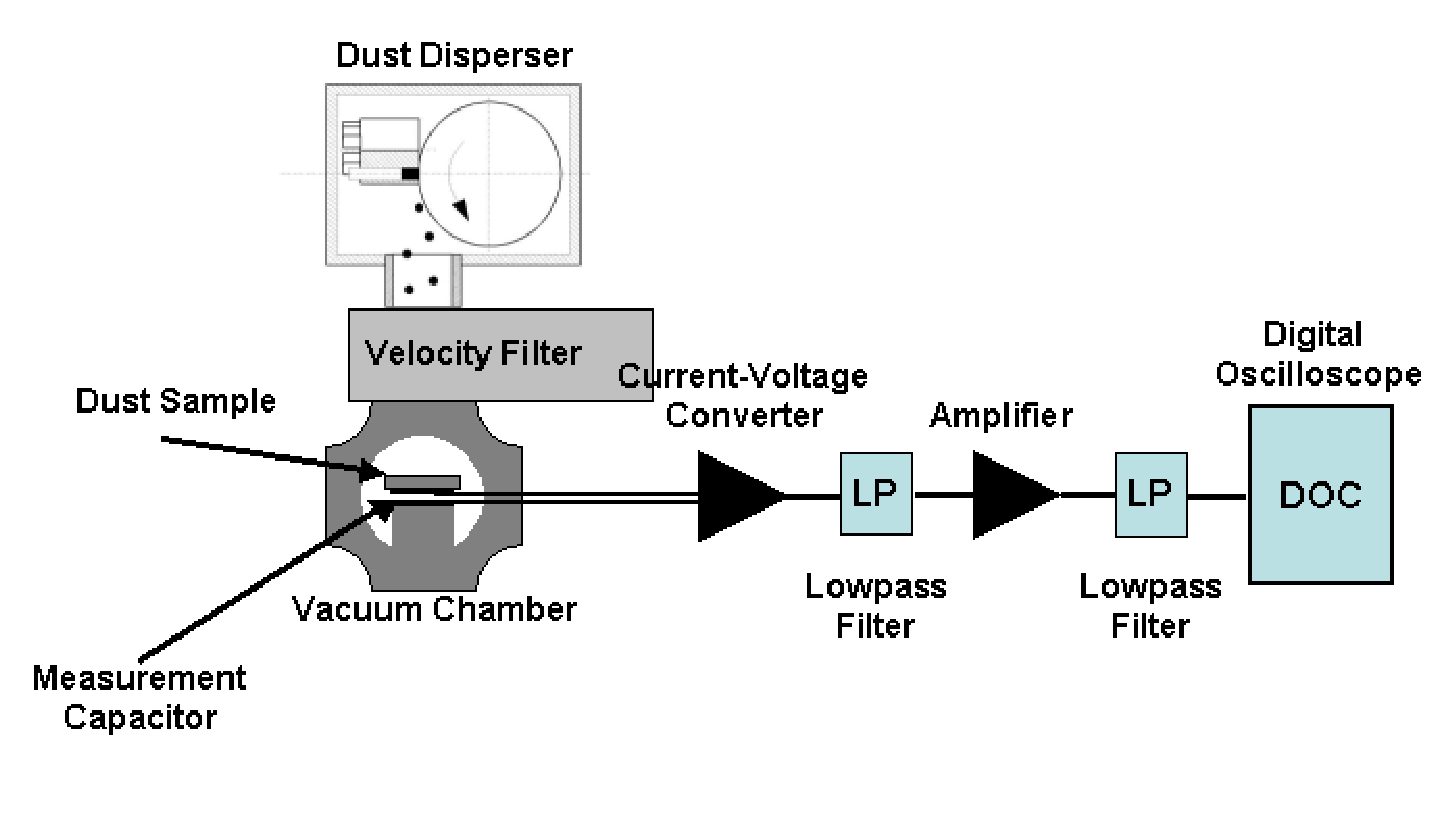
\includegraphics[width=16cm]{b1fig1.eps}}
\caption{\label{fig1blum1}Experimental setup to study the charging
of micrometer-sized dust grains in impacts with cm-sized
high-porosity dust targets.}
\end{figure}


%
% Here follows the own refereed publications by the PIs in relation to
% the project proposed here.
%
\ownpubltitle{Own publications related to the Forschergruppe:}
%
% BELOW IS ONLY AN EXAMPLE OF TWO ENTRIES. SEE THE ADDITIONAL FILES
% SENT TO YOU WITH ALL THE REFERENCES FROM THE VORANTRAG
%
\begin{ownpubl}

\item Blum, J., Wurm, G., Poppe, T. and Heim, L.-O. (1999) Aspects
of Laboratory Dust Aggregation with Relevance to the Formation of
Planetesimals. In: \textit{Laboratory Astrophysics and Space
Research}, Astrophysics and Space Science Library, Vol. 236 (Eds.
P. Ehrenfreund, K. Krafft, H. Kochan, V. Pirronello) Kluwer
Academic Publishers, Dordrecht, 399

\item Blum, J. and Wurm, G. (2000) Experiments on Sticking,
Restructuring and Fragmentation of Preplanetary Dust Aggregates.
\ica, \textbf{143}, 138-146

\item Blum, J., Wurm, G., Kempf, S., Poppe, T., Klahr, H., et al.
(2000) Growth and Form of Planetary Seedlings: Results from a
Microgravity Aggregation Experiment. \prl, \textbf{85}, 2426

\item Blum, J. and Schr\"apler, R. (2004) Structure and Mechanical
Properties of High-Porosity Macroscopic Agglomerates Formed by
Random Ballistic Deposition, \prl, \textbf{93}, 115503

\item Blum, J. (2004) Grain Growth and Coagulation, in:
\textit{Astrophysics of Dust}, ASP Conference Series, Vol. 309
(Eds. A. Witt, G. Clayton and B. Draine), 369-391

\item Heim, L.-O., Blum, J., Preuss, M. and Butt, H.-J. (1999)
Adhesion and Friction Forces Between Spherical Micrometer-Sized
Particles. \prl, \textbf{83}, 3328

\item Heim, L.-O., Butt, H.-J., Schr\"apler, R. and Blum, J.
(2005) Analyzing the Compaction of High-Porosity Microscopic
Agglomerates, Australian Journal of Chemistry, \textbf{58(9)}, 671

\item Krause, M. and Blum J., (2004) Growth and Form of Planetary
Seedlings: Results from a Sounding Rocket Microgravity Aggregation
Experiment. \prl, \textbf{93}, 021103

\item Krauss, O. and Wurm, G. (2005) Photophoresis and the Pile-up
of Dust in Young Circumstellar Disks, \apj, \textbf{630}, 1088

\item Motschmann, U., Sauer, K. and Roatsch, T. (1992) Simulation
of ion acceleration in a charged dust cloud, Geophys. Res. Lett.,
\textbf{19}, 225

\item Poppe, T., Blum, J. and Henning, Th. (1997) Generating a jet
of deagglomerated small particles in vacuum. \textit{Review of
Scientific Instruments\/}, \textbf{68}, 2529

\item Poppe, T., Blum, J. and Henning, Th. (2000a) Analogous
Experiments on the Stickiness of Micron-Sized Preplanetary Dust.
\apj, \textbf{533}, 454-471

\item Poppe, T., Blum, J. and Henning, Th. (2000b) Experiments on
Collisional Grain Charging of Micron-sized Preplanetary Dust.
\apj, \textbf{533}, 472-480

\item Poppe, T. and Schr\"apler, R. (2005) Further Experiments on
Collisional Tribocharging of Cosmic Grains. \aap, \textbf{438}, 1

\item Wurm, G. and Blum, J. (1998) Experiments on Preplanetary
Dust Aggregation. \ica, \textbf{132}, 125

\item Wurm, G., Paraskov, G. and Krauss, O. (2005a) Ejection of
Dust by Elastic Waves in Collisions between Millimeter- and
Centimeter-sized Dust Aggregates at 16.5 to 37.5 m/s Impact
Velocities. \phre, \textbf{71}, 21304

\item Wurm, G., Paraskov, G. and Krauss, O. (2005b) Growth of
Planetesimals by Impacts at ~25m/s. \ica, \textbf{178}, 253-263

\item Wurm, G. and Krauss, O. (2006) Concentration and Sorting of
Chondrules in the Late Solar Nebula. \ica, \textbf{180}, 487-495.

\end{ownpubl}
%
\section{Goals (Ziele)}
Under the conditions of the protoplanetary nebula, larger,
non-fractal dust aggregates are subject to collisions with smaller
dust particles and agglomerates. The impinging projectiles are
either embedded in the target agglomerate (mass gain) or
rebound/fragment upon impact (primary mass loss). The current
understanding is that the growth of pre-planetesimal bodies beyond
a size of $\sim 0.1$~m can no longer be governed by direct
hit-and-stick collisions. Experiments with micrometer-sized
particles have shown (Poppe et al.~2000b, Poppe \& Schr\"apler
2005) that upon impact, target and projectile are charged. A
succession of non-sticking impacts produces a net charge on the
target if there is a preferential charge sign on the projectiles
(as observed by Poppe et al.~2000b). In that case, the escaping
projectiles and/or fragments are deflected in the electrostatic
field after the collisions. If the net charging of the larger
bodies due to a succession of non-sticking impacts is sufficiently
large, escaping projectiles and/or fragments are driven back to
the target surface where they inevitably stick (secondary mass
gain). The here-proposed project will investigate the efficiency
and importance of this electrostatic growth process under
solar-nebula conditions, taking into account state-of-the-art
velocity fields between dust aggregates of different sizes (this
is an input from projects \projklahr{} and \projdul{}) and results
on the ionization state of the surrounding gas (Semenov et al.
2004). The following individual goals have been identified and
will be addressed by project \projblum{}:
\begin{itemize}

\item Determine the number of separated elementary charges as a
function of impact velocity, projectile and target mass,
projectile and target material, projectile and target porosity,
and impact angle.

\item Observation of growth and erosion as a function of impact
velocity, projectile and target mass, projectile and target
material, projectile and target porosity, and impact angle.

\item Determination of coefficients of restitution and ejecta
velocities, angles, and mass distributions.

\item Determination of the charge per ejecta particle in
fragmentation and/or cratering events.

\item Provide input for coagulation equation (i.e.\ input to
project \projdul{}).

\item Modelling of the efficiency of electrostatic secondary
agglomeration under solar nebula conditions, i.e.\ taking into
account realistic collision velocities of the dust and ionization
levels of the gas.

\item Assess the feasibility of electric discharges in the solar
nebula and their importance for chondrule formation.

\end{itemize}

As a side effect, the experiments of project \projblum{} will
result in a much better mapping of the outcomes of mutual
dust-aggregate collisions under the conditions of protoplanetary
disks. Important properties, such as sticking probabilities,
fragmentation probabilities, and fragment size distributions will
be directly available to project \projdul{} for a model refinement
of the overall growth and development towards planetesimals.


\section{Work schedule (Arbeitsprogramm)}
\subsection{Methods}
In the proposed project, impacts of $\rm \mu m$-cm dust
particles/agglomerates into dusty targets of various porosities at
velocities $1 \ldots 100$ m/s are foreseen (see Table
\ref{tab1blum1}). We will extensively make use of existing
experimental hardware in the proposing laboratories (see Sect.
Preliminary work). In the type 1 experiments, single-particle
projectiles will initially be accelerated by the cogwheel dust
disperser (Poppe et al.~1997) with adjacent velocity filter (see
Fig. \ref{fig1blum1}). Parallel to that, a disperser for neutral
dust grains will be developed. Larger dust agglomerates will be
accelerated by recently-developed techniques in the Braunschweig
(stepper motor driven accelerator for high-porosity, mm-sized
agglomerates, type 2 experiments) and M\"unster (cross-bow
accelerator for mm-cm-sized intermediate- to low-porosity
agglomerates, type 3 experiments) laboratories.

\begin{table}[h]
\caption{\label{tab1blum1}Overview of the three experiment types
to be performed in project \projblum{}.}
{\footnotesize %\hspace{-1.0cm}
\begin{tabular}{|l||l|l|l|}
  % after \\: \hline or \cline{col1-col2} \cline{col3-col4} ...
  \hline
  Method & Type 1 & Type 2 & Type 3\\
   \hline
   \hline
  Projectiles & Single micrometer-sized & high-porosity  & intermediate- to low- \\
  & dust grains of arbitrary shape & dust agglomerates & porosity dust agglomerates\\
  \hline
  Targets & low- to high-porosity & low- to high-porosity & low- to high-porosity\\
  & dust agglomerates & dust agglomerates & dust agglomerates\\
  \hline
  Impact velocities & $\sim 1 \ldots 50$~m/s & $\sim 1 \ldots 20$~m/s
  & $\sim 10 \ldots 100$~m/s\\
  \hline
  Observations of & long-distance & high-speed & high-speed \\
  projectile impact & microscopy & camera & camera \\
  \hline
  Measurement of & charge amplifier & deflection of particles &
  deflection of particles\\
  charge transfer & & in electric field & in electric field\\
  \hline
  Additional & Mass gain/loss & Mass gain/loss & Mass
  gain/loss\\
  measurements & of target agglomerate & of target agglomerate & of target
  agglomerate\\
  \hline
\end{tabular}
}
\end{table}

Observations of the impacts are performed by long-distance
microscopic imaging for single-particle type 1 impacts (Poppe et
al.~2000a), and by high-speed imaging techniques for impacting
dust aggregates (type 2 and 3). For these observations, a
high-resolution long-distance microscope (type 1), telecentric
objectives (type 2 and 3), and high-speed cameras (from 500 fps at
1,280 $\times$ 1,024 pixel to 10,000 fps at 65 $\times$ 1,024
pixel) with corresponding illuminations (flash lamps, high-power
halogen lamps, pulsed and continuum lasers) are available at the
proposing laboratories. A plate capacitor for the deflection of
charged ejecta will be used in experiments with projectile
agglomerates (type 2 and 3). This well-established technique
allows the measurements of the coefficients of restitution of
bouncing projectiles and particle trajectories for all ejecta. Due
to the electric field in which the ejecta are travelling, their
acquired charges can be calculated. We expect to be able to
observe electrostatic re-attraction of escaping particles caused
by charge accumulation on the target agglomerate. These
experiments will be extensively performed in the laboratory and
will, if required, also be run in the drop tower under
microgravity conditions. Due to the short experiment time in the
drop tower (up to 9 seconds), an artificial electrical field has
to be applied to simulate the charge accumulation on the target.
The field strength will be adapted to the results of the
long-duration laboratory experiments so that the occurrence of
electrostatic re-accretion can be observed under realistic
experimental conditions. For the experiments with impinging
individual dust particles (type 1), the recently developed
charge-measurement setup will be used (see Fig.\ \ref{fig1blum1}
and Sect.\ 5).

With these experiments, we will try to cover most of the necessary
parameter space. The experimental parameters to be investigated
comprise of (1) porosity of target agglomerate, (2) porosity of
projectile agglomerate (within the limits of the accelerators, see
Table \ref{tab1blum1}), (3) impact velocity, and (4) impact angle
(i.e.\ normal impacts and oblique impacts). Using the experimental
results, a model of the temporal evolution of surface charges of
pre-planetesimal bodies will be developed. The model will include:
\begin{enumerate}
    \item {\bf Charge transfer between projectile and the target
    agglomerate, caused by rebound, fragmentation, or cratering.}\\
    As the
    experiments in this project systematically scan the relevant
    parameter space for collision-induced grain charging, such as
    collision velocity, projectile mass, projectile and target
    material and porosity, we expect to have, at the end of the
    experimental section, a clear view on how many elementary
    charges are separated in which collision.
    \item {\bf Build-up of surface charges on the
    target agglomerate by consecutive non-sticking impacts.}\\
    In the
    second step, we will calculate a typical sequence of impacts
    into an arbitrary dust agglomerate in the protoplanetary
    nebula (this uses extensive input from project \projdul{}) and the
    corresponding accumulation of surface charges (and their
    statistical distribution over the surface), initially not taking into
    account possible discharges by nebula electrons/ions.
    \item {\bf Calculations of the resulting electrical field strength.}\\
    With the
    knowledge of the charge distribution over the surface of the
    dust agglomerate, the near-surface field strength of the
    electric field can be computed. This can be done using the
    COMSOL software package that is available in the Braunschweig
    laboratory.
    \item {\bf Statistical analysis of projectile/fragment
    trajectories within the electrical field in the vicinity of
    the target agglomerate (also taking into account aerodynamic
    drag effects).}\\
    Based upon the measurements of the ejecta
    velocity and angular distribution upon impact, we will compute
    the possible ejecta trajectories to determine the fraction of
    ejecta that are re-accreted by the pre-planetesimal. The
    result of this computation will be the efficiency of
    electrostatic capturing under the conditions of the
    protoplanetary nebula.
    \item {\bf De-charging of the agglomerates by the solar nebula
    gas.}\\
    In the final stage of the modelling effort, we will also take
    into account possible charging/discharging mechanism by the
    electrons/ions in the nebula gas. This effort will be executed
    in close collaboration with D. Semenov at the MPIA and R.
    Nelson/M. Ilgner at QMU who have extensive experience
    in modelling the charge state of the nebula gas.
\end{enumerate}

The final result of the model shall be an assessment about the
importance and efficiency of secondary electrostatic agglomeration
under protoplanetary nebula conditions and a description of the
charging effect in the coagulation equation (input to project
\projdul{}). As a side effect, it is expected that the experiments
and the model will give insight into the occurrence of large-scale
charge separation which might lead to electrostatic discharges
(lightning) in the solar nebula.


\subsection{Schedule}

\subsubsection{First year}
In the first year, the PhD student will build the necessary
hardware components for the three experimental setups described in
Table \ref{tab1blum1} and will extensively test the performance of
the setups. This construction and testing phase will comprise of
the development of a disperser for neutral particles and the
charge measurements in the type 1 experiments, the plate
capacitors and their electrical supplies for the type 2 and 3
experiments, and the observational components for all types of
experiments. In addition to that, software for the data analysis
has to be written. This encompasses trajectory detection
algorithms and the corresponding derivation of the charge-to-mass
ratios of the ejecta. Moreover, ejecta masses are required for the
determination of the charge state of the particles from their
charge-to-mass values. Algorithms for the particle-mass
determination from high-speed images therefore also need to be
developed.

\subsubsection{Second year}
In the second year, systematic laboratory measurements of charging
efficiencies in projectile-target collisions with single-grain and
aggregate projectiles as well as with targets of various
porosities will be performed (type1, type 2, and type 3
experiments). The experiments shall cover the full parameter space
in impact velocity, projectile type, target type, and particle
material. Type 1 and type 2 experiments will be performed in the
Braunschweig laboratory, type 3 experiments will be done in
M\"unster. If the results of the experiments show a considerable
influence of gravity on the results, a series of microgravity
drop-tower experiments on collision-induced grain charging will be
done. The Braunschweig and M\"unster groups have extensive
experience with short-duration microgravity experiments and will
support the development of a miniaturized and autonomous
experimental setup for the drop-tower campaign.

\subsubsection{Third year}
In the final year, a model of charging and discharging of dust
aggregates under the conditions of a protoplanetary nebula shall
be developed following the strategy outlined above. The model
steps comprise of the mapping of the charge transfer between
projectile and the target agglomerate, calculations of the
build-up of surface charges on the target agglomerates by
consecutive non-sticking impacts, computations of the resulting
electrical field strengths, a statistical analysis of
projectile/fragment trajectories within the electrical field in
the vicinity of the target agglomerates, and the de-charging of
the agglomerates by the solar nebula electrons/ions. As a final
result, we expect to compute re-capturing efficiencies of
non-sticking dust particles/aggregates and an assessment on the
importance of this effect for the formation of planetesimals. In
addition, the occurrence of large-scale charge separation will be
calculated and the probability of chondrule melting by electric
discharges will be addressed. Results of the experimental and
theoretical investigations will be published in peer-reviewed
journals.

\subsection{Literature}
%
% Here follows a general literature list related to the topic of the
% proposal, just like a literature list for a scientific paper.
%
% AGAIN ONLY EXAMPLES ARE LISTED NOW
%
\begin{literature}

\item Amelin, Y., Krot, A. N., Hutcheon, I.D. and Ulyanov, A.A. (2002) 
Lead isotopic ages of chondrules and calcium-aluminum-rich inclusions.
\textit{Science} \textbf{297}, 1678--1682.

\item Barge, P. and Sommeria, J. (1995) Did planet formation begin
inside persistent gaseous vortices?, \aap, \textbf{295}, L1

\item Blum, J., Wurm, G., Poppe, T. and Heim, L.-O. (1999) Aspects
of Laboratory Dust Aggregation with Relevance to the Formation of
Planetesimals. In: \textit{Laboratory Astrophysics and Space
Research}, Astrophysics and Space Science Library, Vol. 236 (Eds.
P. Ehrenfreund, K. Krafft, H. Kochan, V. Pirronello) Kluwer
Academic Publishers, Dordrecht, 399

\item Blum, J. and Wurm, G. (2000) Experiments on Sticking,
Restructuring and Fragmentation of Preplanetary Dust Aggregates.
\ica, \textbf{143}, 138-146

\item Blum, J., Wurm, G., Kempf, S., Poppe, T., Klahr, H., et al.
(2000) Growth and Form of Planetary Seedlings: Results from a
Microgravity Aggregation Experiment. \prl, \textbf{85}, 2426-2429

\item Blum, J. (2004) Grain Growth and Coagulation, in:
\textit{Astrophysics of Dust}, ASP Conference Series, Vol. 309
(Eds. A. Witt, G. Clayton and B. Draine), 369-391

\item Blum, J. and Schr\"apler, R. (2004) Structure and Mechanical
Properties of High-Porosity Macroscopic Agglomerates Formed by
Random Ballistic Deposition, \prl, \textbf{93}, 115503

\item Ciesla, F.~J. (2005) Chondrule-forming Processes: An
Overview. In Chondrites and the Protoplanetary Disk (A.N Krot, E.R.D.
Scott, and B. Reipurth, Editors). ASP Conference Series vol.\ 341,
Astronomical Society of the Pacific, San Francisco. pp.\
811-820.

\item Cuzzi, J.~N., Dobrovolskis, A.~R. and Champney, J.~M. (1993)
Particle-gas dynamics in the midplane of a protoplanetary nebula
\ica, \textbf{106}, 102

\item Dominik, C. and Tielens,  A.~G.~G.~M. (1997) The Physics of
Dust Coagulation and the Structure of Dust Aggregates in Space.
\ica, \textbf{480}, 647

\item Gibbard, S.G., Levy, E.H. and Morfill, G.E. (1997), On the
Possibility of Lightning in the Protosolar Nebula, \ica,
\textbf{130}, 517

\item Heim, L.-O., Blum, J., Preuss, M. and Butt, H.-J. (1999)
Adhesion and Friction Forces Between Spherical Micrometer-Sized
Particles. \prl, \textbf{83}, 3328

\item Heim, L.-O., Butt, H.-J., Schr\"apler, R. and Blum, J.
(2005) Analyzing the Compaction of High-Porosity Microscopic
Agglomerates, Australian Journal of Chemistry, \textbf{58(9)} 671

\item Johansen, A., Klahr, H. and  Henning, Th. (2006)
Gravoturbulent formation of planetesimals. \apj, (in press)

\item Krause, M. and Blum J., (2004) Growth and Form of Planetary
Seedlings: Results from a Sounding Rocket Microgravity Aggregation
Experiment. \prl, \textbf{93}, 021103

\item Krauss, O. and Wurm, G. (2005) Photophoresis and the Pile-up
of Dust in Young Circumstellar Disks. \apj, \textbf{630}, 1088

\item Morfill, G., Spruit, H. and Levy, E.H. (1993) Physical
Processes and Conditions Associated with the Formation of
Protoplanetary Disks, In: \textit{Protostars and Planets III}
(Eds. E.~H. Levy, J.~I. Lunine) University of Arizona Press,
Tucson, 939

\item Motschmann, U., Sauer, K. and Roatsch, T. (1992) Simulation
of ion acceleration in a charged dust cloud, Geophys. Res. Lett.,
\textbf{19}, 225

\item Norville, K., Baker, M. and Latham, J. (1991) A Numerical
Study of Thunderstorm Electrification: Model Development and Case
Study. {\it J. Geophys. Res.}, \textbf{96}, 7463

\item Poppe, T., Blum, J. and Henning, Th. (1997) Generating a Jet
of Deagglomerated Small Particles in Vacuum. \textit{Review of
Scientific Instruments\/}, \textbf{68}, 2529

\item Poppe, T., Blum, J. and Henning, Th. (2000a) Analogous
Experiments on the Stickiness of Micron-Sized Preplanetary Dust.
\apj, \textbf{533}, 454-471

\item Poppe, T., Blum, J. and Henning, Th. (2000b) Experiments on
Collisional Grain Charging of Micron-sized Preplanetary Dust.
\apj, \textbf{533}, 472-480

\item Poppe, T. and Schr\"apler, R. (2005) Further Experiments on
Collisional Tribocharging of Cosmic Grains. \aap, \textbf{438}, 1

\item Russell, S.S., Srinivasan, G., Huss, G.R., Wasserburg, G.J. 
and MacPherson, G.J. (1996).  Evidence for widespread $^{26}$Al in the solar
nebula and constraints for nebula time scales.  \textit{Science}
\textbf{273}, 757--762.

\item Schr\"apler, R. and Henning, Th. (2004) Dust Diffusion,
Sedimentation, and Gravitational Instabilities in Protoplanetary
Disks. \apj, \textbf{614}, 960

\item Sekiya, M. and Takeda, H. (2003) Were planetesimals formed
by dust accretion in the solar nebula? \textit{Earth, Planets and
Space\/}, \textbf{55}, 263

\item Semenov, D., Wiebe, D. and Henning, Th. (2004) Reduction of
chemical networks. II. Analysis of the fractional ionisation in
protoplanetary discs. \aap, \textbf{417}, 93

\item Wasson , J.~T. (1996) Chondrule formation: Energetics and
length scales. In: \textit{Chondrules and the protoplanetary disk}
(Eds. R.~H. Hewins, R.H. Jones, E.R.D. Scott) Cambridge University
Press, 45

\item Weidenschilling, S.~J. (1997) The Origin of Comets in the
Solar Nebula: A Unified Model \ica \textbf{127}, 290

\item Weidenschilling, S.~J. and Cuzzi, J.~N. (1993) Formation of
Planetesimals in the Solar Nebula. In: \textit{Protostars and
Planets III} (Eds. E.~H. Levy, J.~I. Lunine) University of Arizona
Press, Tucson, 1031

\item Whipple, F.L. (1966)
  Chondrules: Suggestion Concerning the Origin,
  \sci \textbf{153}, 54

\item Wurm, G. and Blum, J. (1998) Experiments on Preplanetary
Dust Aggregation. \ica, \textbf{132}, 125

\item Wurm, G., Blum, J. and Colwell, J.~E. (2001) Aerodynamical
sticking of dust aggregates. \phre, \textbf{64}, 046301

\item Wurm, G., Paraskov, G. and Krauss, O. (2004) On the
Importance of Gas Flow through Porous Bodies for the Formation of
Planetesimals. \apj, \textbf{606}, 983

\item Wurm, G., Paraskov, G. and Krauss, O. (2005a) Ejection of
dust by elastic waves in collisions between millimeter- and
centimeter-sized dust aggregates at 16.5 to 37.5 m/s impact
velocities. \phre, \textbf{71}, 21304

\item Wurm, G., Paraskov, G. and Krauss, O. (2005b) Growth of
Planetesimals by Impacts at ~25m/s. \ica, \textbf{178}, 253-263

\item Wurm, G. and Krauss, O. (2006) Concentration and Sorting of
Chondrules in the Late Solar Nebula. \ica, \textbf{180}, 487-495.
\end{literature}



\section{External/International collaborations}
\begin{collablist}


\item[MPIA Heidelberg] Dr. D. Semenov will use the results from
this project for revised calculations on the ionization levels and
chemical processes in protoplanetary disks. In addition to that,
Dr. Semenov will model the timescales of charging/discharging of
solid bodies due to electron/ion fluxes in protoplanetary disks to
help assess the importance of electrostatic re-accretion.

\item[Nagoya Univ.] Dr. S. Sirono will use the results of the
impact studies for his mechanical and structural model of
protoplanetary dust aggregates.

\item[Queen Mary Univ. of London] Prof. Dr. R. Nelson, Dr. M.
Ilgner will use the results of this work for their studies on
solar-nebula chemistry and can give valuable input on discharging
timescales.

\end{collablist}



\section{Link to other projects of the Forschergruppe}
\begin{linkproj}

\item[\projtscharn{},\projlattard{}] Projects \projtscharn{} and
\projlattard{} will provide input on abundances of various
minerals to be expected at various parts of the disk. Due to the
detailed chemical and mineralogical modelling in projects
\projtscharn{} and \projlattard{}, much better constraints on the
abundances of the minerals will be available to project
\projblum{}. Thus, the laboratory experiments in project
\projblum{} can always be carried out with dust particles produced
under state-of-the-art knowledge on their relevance.

\item[\projwurm{}] A strong interaction with project \projwurm{}
is envisioned because of common experimental hardware. Both
projects will use identical setups and hardware components so that
a concerted experimentation is required from the logistic as well
as from the scientific point of view. Results of either
experiments can (and possibly will) influence the proceedings of
the respective other work so that a strong interaction between
projects \projwurm{} and \projblum{} is required and foreseen.

\item[B3] Will use experience gained in B3
in using realistic materials such as Mg, Ca, Al silicates and/or Fe-Ni metal
for the planned coagulation experiments.

\item[\projkley{}] The results from the experiments  will provide
input parameters for the SPH code in project \projkley{}, such as
%sticking probabilities and fragmentation outcomes in
%aggregate-aggregate collisions. 
sound speed and elasticity of the porous material.
High-speed, high-resolution
imaging, as used in project \projblum{}, can also help to reveal
the dynamical behavior of interacting dust agglomerates and can be
used to calibrate the SPH simulations.

\item[\projklahr{}] Project \projklahr{} will yield typical impact
velocities for certain aggregate sizes and aggregate properties so
that any findings of project \projklahr{} will influence the
parameter space to be covered in project \projblum{}. On the other
hand results from this project can also influence the modelling in
project \projklahr{} if, under the conditions investigated there,
impact charging plays an important role.

\item[\projdul{}] The experiments in project \projblum{} will
provide valuable input parameters for the dust-dust interactions
for project \projdul{} and will help to define correction terms
for the reaction and coagulation kernel in Smoluchowski's equation
which is the basis for project \projdul{}. Vice versa, project
\projdul{} will be able to predict aggregate abundances, collision
probabilities and collision velocities in protoplanetary disks,
which all are important input parameters for the experiments in
project \projblum{}. As part of the project, an extensive
iteration between laboratory work and modelling efforts is
envisioned.

\item[D1] The textures of agglomerates coagulated under various conditions 
can be directly compared with fine-grained, primitive chondrite assemblages
and cometary dust particles analysed with transmission electron microscopy
/SEM / TOF-SIMS/Nano-SIMS in D1.

\end{linkproj}



\section{\label{persb1}Team members (Zusammensetzung der Arbeitsgruppe)}
%
% NOTE: Only list non-DFG-funded team members.
% NOTE: Also list technical assistants, students etc involved in the project
%
\begin{teamlist}

\item[Blum, J., Prof.~Dr. (C3)]\mbox{}\\
Team leader. Overlooks the experimental and modelling efforts and
supervises the PhD student funded through this project. Provides
extensive expertise in dust collisions, high-speed imaging
techniques, and microgravity experimentation.

\item[Wurm, G., Dr.]\mbox{}\\
Team co-leader. Hosts the PhD student for the type 3 experiments
and for regular visits in M\"unster. Provides extensive expertise
in high-velocity dust impacts and microgravity experimentation.

\item[Kley, W., ~Prof.~Dr. (C4)]\mbox{}\\
Team collaborator. Leads project \projkley{} in which an SPH code
on aggregate-aggregate collisions will be developed. Strong
interactions between \projkley{} and \projblum{} is foreseen to
enhance the output and relevance of both projects.

\item[Motschmann, U., Prof.~Dr. (C3)]\mbox{}\\
Team collaborator. Has widespread experience in modelling
electromagnetic fields and plasmas and will assist in the
development of the theoretical model.

\item[Dullemond, C.P., Dr.]\mbox{}\\
Team collaborator. Is responsible for the transfer of the results
of project \projblum{} to the coagulation code to be developed in
project \projdul{}. Vice versa, valuable input on
aggregate-aggregate collision velocities and frequencies for
project \projblum{} will be provided by \projdul{}.

\item[Klahr, H., Dr.]\mbox{}\\
Team collaborator. Is responsible for the transfer of the results
of project \projklahr{} on aggregate-aggregate collision
velocities and frequencies to project \projblum{}.

\item[Poppe, T., Dr.]\mbox{}\\
Internal collaborator. Dr. Poppe lead the earlier work on impact
charging and will assist the project.

\item[Schr\"apler, R., Dr.]\mbox{}\\
Internal collaborator. Has led the development of the experimental
setup for the type 1 experiments; has extensive experience in
charge measurements and the acceleration and control of
microscopic particles.

\item[Krau{\ss}, O., Dr.]\mbox{}\\
Internal collaborator. Dr. Krau{\ss} has extensive experience in
dust-impact research in the laboratory and in the drop tower.

\item[Stoll, B.]\mbox{}\\
Electronics Engineer. Will assist in the experimental setups on
charge measurements.

\item[Jelting, E.]\mbox{}\\
Electronics Engineer. Will assist in the experimental setups on
charge measurements.

\item[Gebauer, K.]\mbox{}\\
Mechanics Technician. Will assist in the construction of new
experimental hardware.


\end{teamlist}
\vspace{1em}



\section{Funding requested}
The following table gives the full overview of requested
funding:\vspace{1\baselineskip}\\
%
% The table that follows is the overview over the full requested
% funding, including the positions, travel, consumables and ``other
% costs'' (which might include transportation costs of radioactive
% material or the rent of a drop tower or such).
%

\centerline{
\begin{tabular}{||l|l|l|l||} \hline \hline & Year 1 & Year 2 &
Year 3 \\ \hline %
Personnel (1 PhD-students: E13/2)   & \hfill 24,000  & \hfill 24,000 & \hfill 24,000 \\
Equipment                           & \hfill 12,269  & \hfill -      & \hfill - \\
Consumables                         & \hfill 9,000   & \hfill 7,000  & \hfill 6,000 \\
Travel                              & \hfill 4,000   & \hfill 5,600  & \hfill 5,600 \\
Other costs                         & \hfill -       & \hfill  -     & \hfill  -    \\
\hline
{\bf Total:}                        & \hfill 49,269 & \hfill 36,600 & \hfill 35,600 \\
\hline \hline
\end{tabular}
}

\vspace{1em}

{\noindent Below these costs are explained in more detail:}

\subsection{Personnel (Personalbedarf)}
\begin{teamlist}
\item[PhD-Student (E13/2)]\mbox{}\\
The PhD student shall perform independent experimental and
theoretical research to reveal the importance and efficiency of
electrostatic agglomeration.
\end{teamlist}

\subsection{Equipment (Ger\"ate)}

For the experiments to be performed within project \projblum{},
high-vacuum equipment is mandatory. Due to possible electrical
discharges, a mechanical pump is not sufficient, but needs to be
augmented by a turbo-molecular pump. A complete setup is available
from Leybold (PT 50) at a cost of EUR 7,923. A dedicated vacuum
chamber, consisting of a CF-100 double-cross-piece (EUR 1,699 at
Leybold) and 6 CF-100 flanges (EUR 647 at Leybold), will be
purchased for the housing of the experiment. Vacuum gauges are
available at the Braunschweig laboratory at no cost. A
work-station PC with image analysis software for the PhD student
is required. The cost of this PC will be approximately EUR 2,000.

Estimated cost:\vspace{1\baselineskip}\\
\centerline{
\begin{tabular}{||l|l|l|l||} \hline \hline & Year 1 & Year 2 &
Year 3 \\ \hline %
High-vacuum pump &  \hfill 7,923 & \hfill - & \hfill - \\
Vacuum chamber & \hfill 2,346 & \hfill -& \hfill -\\
PC &  \hfill 2,000 & \hfill - & \hfill - \\
\hline
{\bf Total:}    & \hfill 12,269 & \hfill - & \hfill - \\
\hline \hline
\end{tabular}
}


\subsection{Consumables (Verbrauchsmaterial)}
The experiments require rather large amounts of dust. As some
experiments shall be used for calibration purposes of the SPH code
(project \projkley{}) and linking to earlier works, they will
consume spherical, mono-disperse, micrometer-sized $\rm SiO_2$
particles. We estimate the annual cost for this dust to EUR 1,500
(corresponding to 100 g). Other dust types are somewhat cheaper
but will be consumed in higher quantities so that an additional
estimated EUR 4,500 will be required. For the connection of the
high-vacuum pump to the experiment chamber, vacuum components
(flanges etc.) are required which will cost EUR 2,000 (in year 1
only). For the development of a disperser for neutral dust
particles in the type 1 experiments, workshop material (metals,
tools) is required in year 1 and year 2. We estimate the annual
costs to be EUR 1,000.

Estimated cost:\vspace{1\baselineskip}\\
\centerline{
\begin{tabular}{||l|l|l|l||} \hline \hline & Year 1 & Year 2 &
Year 3 \\ \hline %
Dust particles &  \hfill 6,000 & \hfill 6,000 & \hfill 6,000 \\
Vacuum equipment& \hfill 2,000 & \hfill -& \hfill -\\
Workshop material&\hfill 1,000 & \hfill 1,000 & \hfill -\\
\hline
{\bf Total:}    & \hfill 9,000 & \hfill 7,000 & \hfill 6,000 \\
\hline \hline
\end{tabular}
}

\subsection{Travel expenses in addition to Project Z (Reisekosten)}
%
% Here only travel expenses not related to usual regular Forschergruppe
% meetings and the overall per capita budget for conferences.
%
Regular project meetings with the participants of this projects
are required. We estimate that two full-day meetings per year (at
various locations) are required. For each person, the cost per
meeting will be EUR 150 for the train, EUR 50 for hotel and EUR 50
for per diem, i.e.\ a total of EUR 250. For each meeting, the
number of travellers is estimated to be three so that a total of
EUR 750 is required. In addition to that, two regular one-week
preparation visits per year by the PhD student to M\"unster (year
1, year 2) and Heidelberg/T\"ubingen (year 3) are required. Each
trip will cost EUR 150 (train) + EUR 100 (per diem) + EUR 200
(hotel) = EUR 450. Additionally, the PhD student is required to
make extensive (three-week) measurement campaigns in M\"unster.
Each campaign will cost EUR 200 (rental car) + EUR 500 (per diem)
+ EUR 900 (hotel) = EUR 1,600. A drop tower campaign demands a
three-week presence in Bremen; thus, the costs will be equivalent
to that of the other three-week campaigns (EUR 1,600). Two
drop-tower campaigns (years 2,3) are foreseen.

Estimated cost:\vspace{1\baselineskip}\\
\centerline{
\begin{tabular}{||l|l|l|l||} \hline \hline & Year 1 & Year 2 &
Year 3 \\ \hline %
Regular meetings &  \hfill 1,500 & \hfill 1,500 & \hfill 1,500 \\
Preparation visits& \hfill 900 & \hfill 900 & \hfill 900 \\
Measurement campaign & \hfill 1,600 & \hfill 1,600 & \hfill 1,600 \\
Drop-tower campaign & \hfill - & \hfill 1,600 & \hfill 1,600 \\
\hline
{\bf Total:}    & \hfill 4,000 & \hfill 5,600 & \hfill 5,600 \\
\hline \hline
\end{tabular}
}

\subsection{Other costs (Sonstige Kosten)}
There are no others costs.
%%Publication costs will amount to EUR 1,000 for the years 2 and 3.

%Estimated cost per year:\vspace{1\baselineskip}\\
%\centerline{\begin{tabular}{|p{15em}|p{10em}|p{7em}|}
%\hline
%?  & \hfill ? & \hfill ? \\
%\hline
%\end{tabular}}

%Estimated cost:\vspace{1\baselineskip}\\
%\centerline{
%\begin{tabular}{||l|l|l|l||} \hline \hline & Year 1 & Year 2 &
%Year 3 \\ \hline %
%Publication costs & \hfill - & \hfill 1,000 & \hfill 1,000 \\
%\hline
%{\bf Total:}    & \hfill - & \hfill 1,000 & \hfill 1,000 \\
%\hline \hline
%\end{tabular}
%}


\section{Preconditions for carrying out the project at home institution}
%
% This is one of the main subsections of a DFG Normalverfaren proposal.
% Several of the subsubsections in this subsection we have placed in their
% own subsections above (like team members, collaborations). What remains
% are the following three subsections. For those not familiar with these,
% we refer to the DFG Merkblatt on Normalverfahren-proposals.
%
\subsection{\label{equipb1}Scientific equipment available (Apparative Ausstattung)}
%
% Please list those larger instruments available to you for the project (if
% applicable also larger computer equipment in case you need substantial
% amounts of computer time).
%
In the Braunschweig and M\"unster laboratories, the following
equipment is available for this project at no cost:
\begin{itemize}

\item High-speed, high-resolution camera Mikrotron 1310, from 500
frames per second at 1,280 $\times$ 1,024 pixel to 10,000 frames
per second at 65 $\times$ 1,024 pixel for the type 1-3 laboratory
experiments.

\item Ruggedized high-speed, high-resolution camera Vossk\"uhler
HCC, from 462 frames per second at 1,024 $\times$ 1,024 pixel to
1,386 frames per second at 256 $\times$ 1,024 pixel for drop-tower
experiments.

\item Long-distance microscope with 80 mm working distance and
$\sim 1~\rm \mu m$ resolution for the type 1 experiments.

\item Telecentric objective lenses for the type 2 and type 3
experiments.

\item High-speed flash lamps (up to 1,000 per second) with
ultrashort ($\sim 1~\rm \mu s$) flash duration for type 1-3
experiments.

\item Continuous and pulsed laser diode for type 1 experiments.

\item Halogen lamps for type 2-3 experiments.

\item High-sensitivity charge measurement equipment (under
construction), comprising of charge amplifier and data recorder
for type 1 experiments.

\item High-voltage power supply for type 2-3 experiments.

\item Cogwheel-type dust deagglomerator and accelerator (up to
$\sim 50$ m/s) for preliminary type 1 experiments.

\item Velocity filter for the precipitation of unwanted particle
sizes and velocities in type 1 experiments.

\item Stepper motor driven accelerator (under construction) for
high-porosity dust aggregates and velocities up to $\sim 20$ m/s
(type 2 experiments).

\item Cross-bow accelerator for low- to medium-porosity dust
aggregates and velocities up to $\sim 100$ m/s (type 3
experiments).

\item High-precision balance (Sartorius MC 210 P; measurement
sensitivity $10^{-5}$~g at 200~g maximum mass) for target mass
determination.

\item COMSOL Multiphysics software with Earth Science Module and
Electromagnetics Module for the modelling of (1) the deflecting
electric fields for the charge measurements and of (2) the
electric fields around protoplanetesimals.

\item Vacuum gauges for high- and low-vacuum conditions.

\item Additional flash lamps, scales, and equipment to run type 3
experiments in M\"unster.

\end{itemize}


\subsection{Institution's general contribution (Laufende Mittel f\"ur Sachausgaben)}

Besides the scientific instrumentation (see Sect. \ref{equipb1})
and personnel costs (see Sect. \ref{persb1}), the proposing
institutions will support this project with EUR 1,000.

%
% Please state the annual fund for consumables which comes from the
% institution's budget or any other third party  (please list separately) to
% pay for the research for which your project is part of.  Use estimates where
% applicable.
%

%We estimate that the running costs per year of our equipment
%are:\vspace{1\baselineskip}\\
%%
%\centerline{\begin{tabular}{|p{18em}|p{7em}|p{7em}|}
%\hline
%?                & \hfil ? & \hfil ? \\
%\hline
%?                & \hfil ? & \hfil ? \\
%\hline
%\end{tabular}}



